\begin{center}
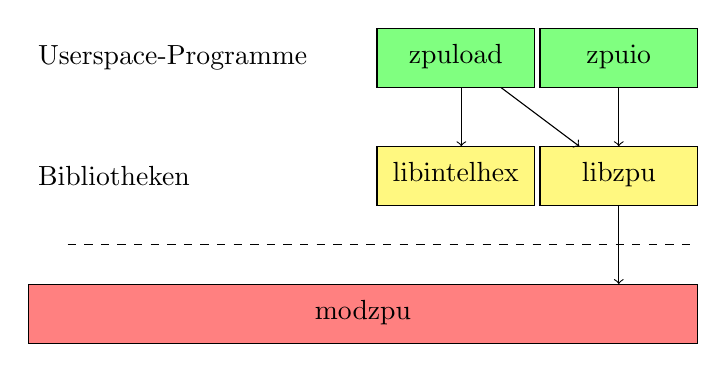
\begin{tikzpicture}
	\usetikzlibrary{positioning}
	\tikzstyle{node}=[anchor=mid,text centered,minimum height=2em];
	\tikzstyle{app}=[draw,fill=green!50,rectangle]
	\tikzstyle{lib}=[draw,fill=yellow!50,rectangle]
	\tikzstyle{dri}=[draw,fill=red!50,rectangle]
				
	\draw [lib] (6,0.5) rectangle +(2,0.75) node [node,midway] {libzpu};
	\draw [lib] (4cm-2pt,0.5) rectangle +(2,0.75) node [node,midway] {libintelhex};
				
	\draw [dri] (-0.5,-0.5) rectangle +(8.5,-0.75) node [node,midway] {modzpu};
	\draw [app] (6,2) rectangle +(2,0.75) node [node,midway] {zpuio};
	\draw [app] (4cm-2pt,2) rectangle +(2,0.75) node [node,midway] {zpuload};
					
	\draw [dashed] (0,0) -- (8,0);
	\draw [->] (7,0.5) -- (7,-0.5);
	\draw [->] (7,2) -- (7,1.25);
	\draw [->] (5,2) -- (5,1.25);
	\draw [->] (5.5,2) -- (6.5,1.25);
				
	\node [anchor=west] at (-0.5, 2.375) {Userspace-Programme};
	\node [anchor=west] at (-0.5, 0.875) {Bibliotheken};
\end{tikzpicture}
\end{center}